\documentclass[11pt]{article}
\usepackage[numbers, sort&compress]{natbib}
\usepackage{amsmath}
\usepackage{amssymb}
\usepackage[ruled,linesnumbered]{algorithm2e}	
\usepackage{multirow}
\usepackage{hyperref}
\usepackage{float}
\usepackage{graphicx}
\usepackage[table,xcdraw]{xcolor}
\usepackage{booktabs}
\usepackage{caption}
\usepackage{tikz}
\usepackage{array}
\hypersetup{
	colorlinks,
	linkcolor=blue,
	filecolor = blue,
	citecolor=red,
	urlcolor=blue
}\setlength{\belowcaptionskip}{-15.0pt}
\title{Image Segmentation of coin and non-coin pixels using Gaussian Mixture Models}
\author{Kenan Karavoussanos}
\begin{document}
	
	
	
	\maketitle
	
	\newpage
	
	
	\section{Introduction}
	

	\subsection{Aim} The aim of this work is to develop a Gaussian Mixture Model for the purpose of Image Segmentation. We are given a set of training images and binary mask images, where the mask image indicates whether a pixel is a coin or non-coin pixel. The model takes in a set pixels as input and outputs the label of each pixel. This label array is then reshaped into the original image dimensions and produces as binary mask, with coins pixels white and non-coin pixels black. 
	
	\subsection{Gaussian Mixture Models} A Gaussian Mixtures Model(GMM) is a probabilistic model that makes the assumption that all data is produced via a linear combination of a finite number Gaussian Distributions. Thus the likelihood of our data is modeled as follows:

	$$\mathbb{P}( \underline{x} \lvert \underline{\theta}) = \sum_{i=1}^{K} \lambda_i Norm_{\underline{x}}[\underline{\mu}_i, \underline{\Sigma}_i]$$

	Where $\underline{\lambda}$ and each $\underline{\mu}_i, \underline{\Sigma}_i$ are parameters learned via the \emph{Expectation Maximization} algorithm. Once these parameters are learned, we use Bayes' Rule for inference, i.e classifying each pixel. 
	
	
	\subsubsection{Expectation Maximization for Gaussian Mixture Models}
	
		
		Expectation Maximization(EM) is a general iterative method for fitting the parameters of a statistical model, that depends on a number of hidden variables. We avoid discussing Expectation Maximization in general and instead view it in the context of Gaussian Mixture Modeling. The Expectation Step, involves calculating the responsibility of each distribution for each data point, that is, the responsibility of the $k^{th}$ distribution for the $i^{th}$ data point is given by
		
		$$ r_{ik} = \frac{ \lambda_{k}Norm_{\underline{x}_i}[\underline{\mu}_k, \underline{\Sigma}_k]}{\sum_{j=1}^{K} \lambda_{j}Norm_{\underline{x}_i}[\underline{\mu}_j, \underline{\Sigma}_j]}$$
		
		\paragraph{} The Maximization step involves fitting the model parameters with respect to the new set of responsibilities calculated in the expectation step. This, conveniently, takes the form of the following update rules:
		
		$$\lambda^{[t+1]}_{k} = \frac{\sum_{i=1}^{I} r_{ik}}{\sum_{j=1}^{K}\sum_{i=1}^{I} r_{ij}}$$
		
		$$\underline{\mu}^{[t+1]}_{k} = \frac{\sum_{i=1}^{I} r_{ik}\underline{x}_i}{\sum_{i=1}^{I} r_{ik}}$$
				
$$\underline{\Sigma}^{[t+1]}_{k} = \frac{\sum_{i=1}^{I} r_{ik}(\underline{x}_i - \underline{\mu}^{[t+1]}_{k})(\underline{x}_i - \underline{\mu}^{[t+1]}_{k})^{T}}{\sum_{i=1}^{I} r_{ik}}$$
		
	
	\section{Design Details}
	
	\subsection{Dataset}
	
	We are given a set of 100 training images and masks. Each training image is 1280 x 960 pixels. Due to computational time constraints, each training image and mask was downscaled by a factor of 0.25, resulting in images and masks of 320 x 240 pixels.
	Furthermore, we limited our training dataset to the first five images, again for the purposes of limiting computation time. 
	
	\subsection{Color Space} We make use of the HSV color space in this work. The Value channel in this color space indicates the brightness of the image. Within the context of the input data, we observe that desk pixels have low brightness and coins pixels have high brightness, as such the Value of each pixel represents a good discriminative feature for the problem of binary classification. 
	
	\subsection{Covariance Form} We make use of diagonal covariance matrices in this work. That is, we make the assumption that each channel of our color space in independent of the other. This enables us to reduce computational time by decreasing the number of trainable parameters in our covariance matrices from $K \times D \times D$ to $K \times D$ where $K$ is the number of  Gaussian distributions in our mixture model and $D$ is the number of channels in our color space. Additionally, this allows us to replace the matrix multiplication in the calculation of $\underline{\Sigma}^{[t+1]}_{k}$ in the Maximization step, with the element-wise square of our covariance vector.

	\subsection{Inference}
	
		We train two mixture models over the coin pixels and desk pixels in our dataset, respectively. This provides the class conditional likelihood of our data. These likelihoods are substituted into Bayes' Rule to produce the posterior distribution over our labels, given our data and fit model parameters. We then make use of Otsu's Method to find a suitable threshold for classification.
	
	\section{Experiments}
			
	\subsection{Experimental Setup}	
	\paragraph{}We analyze the Training Precision, Recall and Accuracy after each iteration of the EM algorithm, to a maximum of 10, and do this for $K = 2, 3, ..., 10$. This enables us to analyze the behavior of each model while it trains. Due to the large class imbalance, the most significant performance metric is the precision. We limit the EM algorithm to a fixed number of iterations due to the computational time cost of each iteration.
		
		\paragraph{}We then select the highest precision model $(K = 10)$ and train it for 20 iterations and assess its test precision, recall and accuracy.
		
	\subsection{Results}
	
		\subsubsection{Figures}
		See appendix


	\subsubsection{Discussion}
	
	From figure 1 we can see Training Precision has a positive correlation with the number of Expectation Maximization iterations. This confirms that the model is learning, however, the precision ranges from 50\% to 62\% which is poor. This is potentially solved by running further iterations of the EM algorithm. We can observe that there is positive correlation with K and precision which is expected. From figure 2 we observe that recall is consistently above 93\% peaking at 96\%. We can also see similarly high accuracy from figure 3, ranging from 93\% to 96\%. The high accuracy and recall values can be explained by the class imbalance in the dataset. When evaluating the test performance on the final fit GMM with K = 10, we achieve test precision of 74.2\%, recall of 96.2\% and accuracy of 97.27\%. The test precision value shows that the model generalizes to unseen data. 

\section{Appendix}

	\begin{figure}[H]
	
	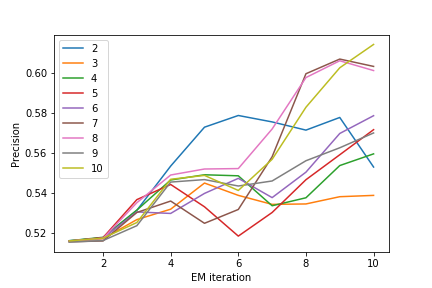
\includegraphics[width=\textwidth, keepaspectratio]{Precision.png}
	
	\caption{Training Precision versus EM Iteration for varying number of distributions K}
\end{figure}

\begin{figure}[H]
	
	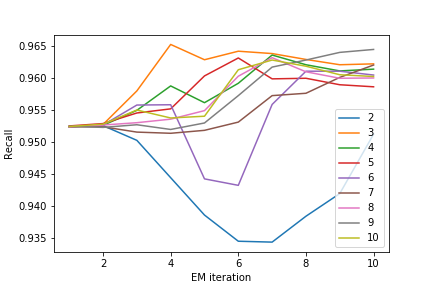
\includegraphics[width=\textwidth, keepaspectratio]{Recall.png}
	\caption{Training Recall versus EM Iteration for varying number of distributions K}
\end{figure}
\begin{figure}[H]
	
	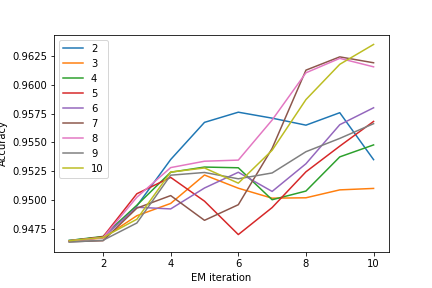
\includegraphics[width=\textwidth, keepaspectratio]{Accuracy.png}
	\caption{Training Accuracy versus EM Iteration for varying number of distributions K}
\end{figure}
\end{document}







